\section*{Bilag 1: 7-bit tegnsæt}
\begin{figure}[H]
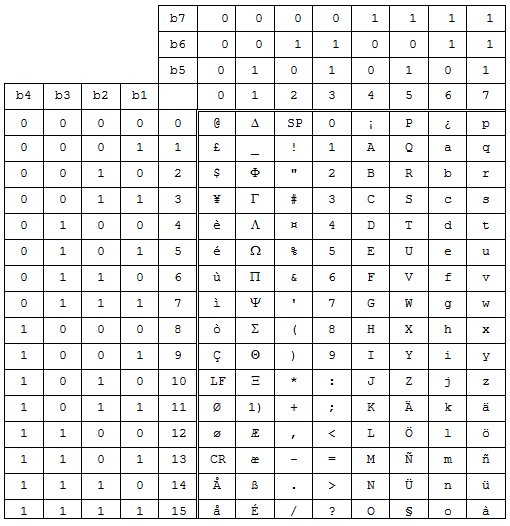
\includegraphics []{Billeder/tegnsaet.png}
\caption {Her ses skemaet for bit 7 tegnsættet. Ved 0x1b ses tegnet 1), der er et escape tegn til den ekstra tabel, som ses på figur \ref{tegnsaet2}}
\label {tegnsaet}
\end{figure}

\section*{Bilag 2: 7-bit tegnsæt del 2}
\begin{figure}[H]
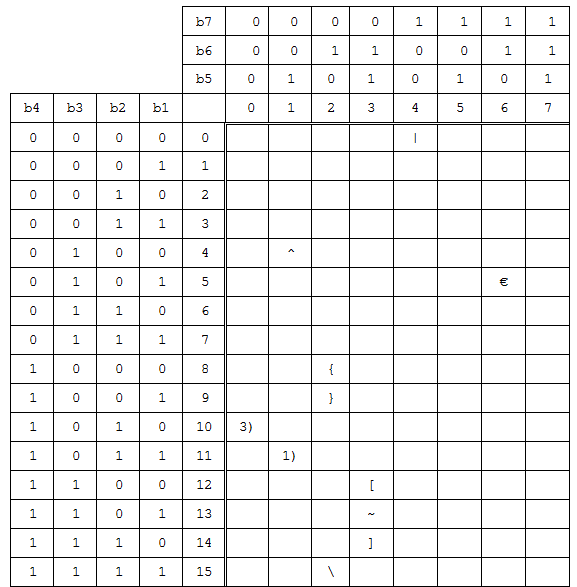
\includegraphics []{Billeder/tegnsaet2.png}
\caption {Den ekstra tabel for bit 7 tegnsaettet. Det samme tegn 1), er her et escape tegn som er reserveret hvis en ny ekstra tabel introduceres. Tegnet 3) er et form feed tegn, som er et escape tegn der starter en ny side}
\label {tegnsaet2}
\end{figure}

\section*{Bilag 3: Mest brugte tegn i dansk Wikipedia}
\begin{figure}[H]
\centering
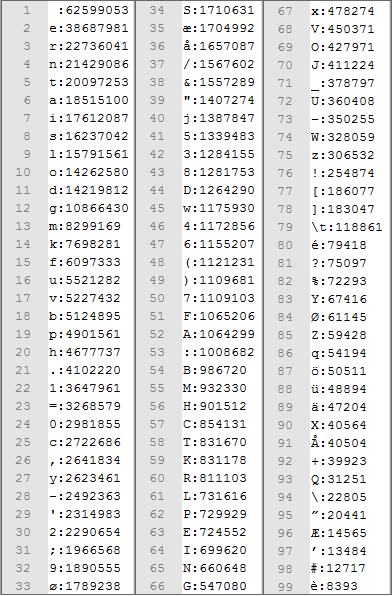
\includegraphics []{Billeder/wikiBilag.png}
\caption {Tabellen viser top 100 over mest brugte tegn i over 340.000 danske Wikipedia artikler}
\label {wikiAnalyse}
\end{figure}

\section*{Mest brugte tegn i vores SMS-analyse}
\begin{figure}[H]
\centering
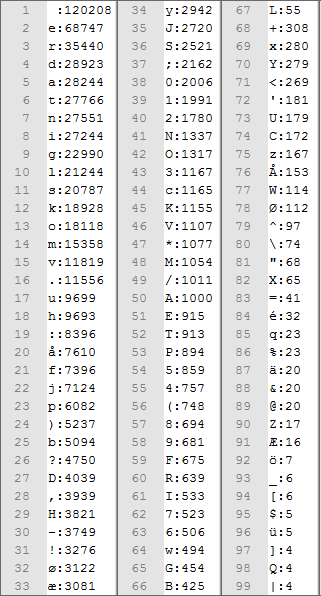
\includegraphics []{Billeder/SMSbilag.png}
\caption {Figuren viser top 100 over mest brugte tegn fra vores SMS analyse af over 13.000 SMS beskeder.}
\label {SMSanalyse}
\end{figure}

